\subsection{Specification Environment}\label{sec:envfeatures}
\noindent
We identified the following distinguishing environment characteristics that are related to the specification of missions.
%The value in brackets indicates the number of environments offering the optional feature out of 29. While simulator (10/29), multiLanguageSupport (13/29) and debugging (13/29) features are optional. Much as it is desirable to have to have a debugger and a simulator, not all the environments supported these features. 

\begin{figure}[t]
     \centering
    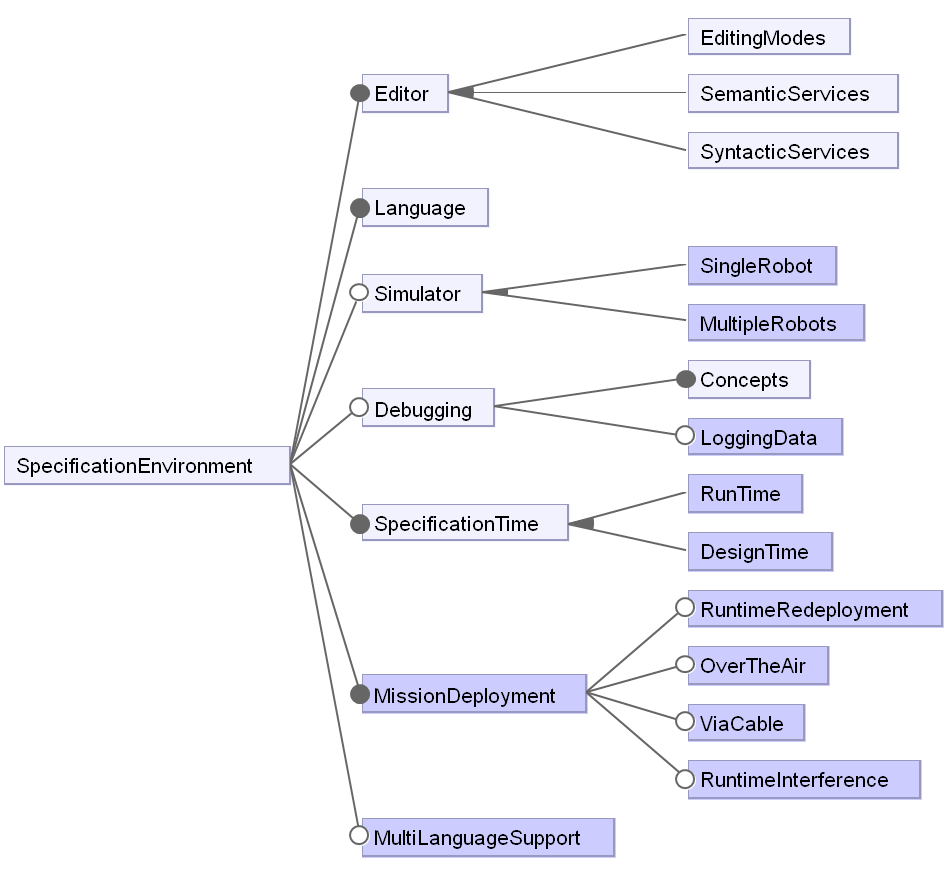
\includegraphics[width=\columnwidth]{fig/toplevelfeatures.png}
		  \smash{\begin{minipage}{8.3cm}
						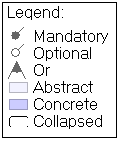
\includegraphics[width=.18\columnwidth]{fig/legend.png}
						\vspace{2.3cm}
						\end{minipage}
			}
			\vspace{-.3cm}
      \caption{Overview of all features identified%\tb{was my version, please update, but please fix the naming of some features as I did in this figure}
      }
      \label{fig:featuremodel}
			\vspace{-.4cm}
\end{figure}

\newcommand{\fsyntacticservices}{\f{SyntacticServices}}
\newcommand{\fsemanticservices}{\f{SemanticServices}}
\newcommand{\feditingmode}{\f{EditingMode}}

\parhead{\feditor.} While the editor tooling in our environments of course offers typical editor capabilities (e.g., copy, paste, or undo), we found the following distinguishing characteristics represented by the features \fsyntacticservices, \fsemanticservices, and \feditingmode, as follows.

%Besides the basic editor features such as cut, paste, and redo; we also found syntactic services, semantic services, and editing modes as editor features.

Syntactic services (feature \fsyntacticservices) support developers creating a correct Abstract Syntax Tree (AST) of the mission specification, according to the language's abstract syntax. We found various of such services. Especially, syntax highlighting with coloring is available in all environments.  %todo: verify \flyaq and \tivipe
We furthermore found a range of convenience services, such as an outline view for navigation support (e.g., in \picaxe), syntactic completion templates for users (e.g., in \edison and \ardublockly), and automated formatting (e.g., in \arcbotics, \robotmesh, and \vex).

%and invalid variable name \minibloq -> isn't that a kind of error highlighting?

%restructuring, aligning or lay-outing \cite{erdweg2013languageworkbenches} as seen in \robotmesh, \vex  -> explain what that is (didn't find in the spreadsheet)

%offer support for correct expression structure, as defined by a language to support specification of missions. The syntactic services captured include; language specific syntax coloring and symbol shapes in graphical notations, were evident in almost all the environments studied with exception of \flyaq and \tivipe where the authors were not sure. -> symbol shapes is not a syntactic service

Semantic services (feature \fsemanticservices) support developers creating an abstract syntax tree that is semantically meaningful, inspired by the definition of semantic services in~\citet{erdweg2013languageworkbenches}. We identified: auto-completion (e.g., in \vex, \trik, \picaxe, \edison);  live translation where generated code is displayed side-by-side to the graphical notation (e.g., in \easyc); error highlighting (e.g., in \edison, \aseba, \vex, \robotmesh, \blocklyprop, \minibloq, and \easyc) directly on the mission specification, for instance the indication of compile errors at the respective lines in \blocklyprop, or as a pop-up help (e.g., in \edison, \missionlab, and \choregraphe). However, more than half of the environments did not offer any semantic services. % -> verify

%and auto-help when activated enables automatic reference when blocks are selected ~\cite{ozobot} as seen in \ozoblockly, \edison.

Finally, the editing mode (feature \feditingmode) typically classifies into parser-based and projectional editing\,\cite{voelter2014projectional,berger2016pe}. In the former, the user edits the source code, which is represented by a sequence of characters in a free form. In the latter, the user's editing gestures directly change the underlying AST, which is projected using projection rules into a user-observable syntax, which can resemble textual and visual syntax, or a combination of both. \Figref{fig:easyc-sidebyside} illustrates the power of projectional editing in the environment \easyc, showing visual and textual syntax side-by-side. The typical continuous enforcement of a correct AST in projectional editing guides users towards correct mission specifications, which can also be seen as a semantic service. For all our environments, given the restriction to visual languages, every environment provides a projectional editor. However, three also offer textual languages, to be used in parallel as an alternative, relying on parser-based editing: \aseba, \vex, and \turtlebot.% and \robotc\tb{where is that stated for \robotc? can you give me the exact source?}.

\parhead{\fmultilang.} A total of 13 of the environments offer multiple languages to specify missions. While at least one visual language is supported (according to our selection criteria), many environments offer at least one more language. For instance, \picaxe provides two visual languages, based on a \fflowchart and a \fblockly notation, respectively. Moreover, it offers a language with a textual syntax in the style of the programming language Basic and it offers the use of JavaScript.


%, and projectional mode where, the program has a standard fixed layout. In projectional editors are structured editors in which a developer works directly on the bstract syntax tree(AST) \cite{berger2016pe}, coding is done using intuitive onscreen visuals.
%\parheadit{Example} Of the 29 environment studied, only four support parser based editing mode; \aseba, \vex, \turtlebot and \robotc. This finding is not surprising since in the selection criteria, the study is biased to end-user supporting environments. 

\parhead{\fsimulator.} Ten of our environments provide simulation support to test missions before they are executed. This helps in ensuring safety and creating opportunities to train users without necessarily using the actual robots. One of the simulators, that of \missionlab, even supports multiple robots.
%The simulator either support single robot at a time or more than one robot and/or robot type. -> which ones? do we have evidence that multiple robots are supported by at least one simulator?

\parhead{\fdebugging.} A total of 13 of our environments offer debugging support. We found a variety of debugging tools, including the live monitoring of sensor data, the state of actuators, and variables in the environments \picaxe, \aseba, \trik, \flyaq, \easyc, and \edison. The \edison environment  offers a box to control inputs, manipulate data, and monitor the use of variables. % -> what was 'bug-box'?
Interestingly, \makecode communicates execution traces via sound and printing text between the execution of program blocks. % -> not so clear
We also found the typical break-point mechanism to hold and monitoring executions (e.g., in \robotmesh).
Furthermore, \openroberta provides a `check box' in the \texttt{start block}, and when checked, it displays current values of the connected sensor data during program execution. %menu\tb{please give me the exact source of this information (paper and position)} to confirm that the mission specification the robot's configuration matches---important since the environment supports different types of robots. 
% -> this all needs to be verified

\parhead{\fspectime.} Missions are specified either at design time or run-time. Design-time specification provides all the details about the mission before the execution starts.
 %which calls for explicit modeling of the environment.
All environments support design-time specification. A few environments (namely \turtlebot, \sphero, and \choregraphe), however, also offer some remote-control functionality to intercept the mission execution at runtime. % -> verify
%with the exception of \turtlebot, \sphero and \choregraphe. For instance, in \choregraphe, different missions can be deployed on the robot at run-time. \sphero supports interaction with the robot at run-time using a Bluetooth connection. % -> I think this is wrong

\parhead{\fdeployment.} Missions, once specified, are transferred to the robots for execution. Not surprisingly, we found different combinations of media to transfer missions, including USB cable, Ethernet cable, custom cable, as well as WiFi and Bluetooth connections.
 %Environments such as \trik and \lego support USB, WiFi, and Bluetooth connections for deployment over-the-air. While \tello missions can be deployed using Bluetooth, and Wi-Fi. Most environments use either USB, Ethernet or a custom cable to deploy missions to robots. \\ 


% \textbf{items removed}
% \begin{itemize}
%     %\item file access
%     \item time has been merged as a measure of action under action types
%     \item example as an example of syntax services
%     \item formal notation (generic code, natural language text, forms, blocks, icons) and secondary notation (syntax highlighting, size, notation color, comments) as concrete features of notation.
%     \item behavior concepts with concrete features like discrete behavior and continuous behavior from language features
%     \item robot with single/multi-robot mission (swarm/team), multi-robot, single robot, robot types and connection and multi-robot types as concrete features
%     \item Mission deployment support; hardware requirements and software requirements
%     \item debugging environments; simulation, actual robot
%     \item modeling concepts and explicit modeling of environment 
% \end{itemize}
